\documentclass[a4paper,11pt, oneside]{phdthesis}
%
% for customizing the page size
\usepackage[vcentering,dvips]{geometry}
\geometry{papersize={190mm,260mm},margin=2.5cm, bottom=2.5cm, top=2.5cm}
%
%using fancy header for customizing the page header
\usepackage{fancyhdr}
\pagestyle{fancy}
\fancyhf{}
%
\renewcommand{\chaptermark}[1]{\markboth{\MakeUppercase{#1}}{}}
\renewcommand{\sectionmark}[1]{\markright{\MakeUppercase{#1}}{}}
\renewcommand{\headrulewidth}{3.0pt}
%
\mainmatter{}
\fancyhead[RE,LO]{{\footnotesize\rightmark} }
\renewcommand{\headrulewidth}{0.5pt}
%
\setlength{\headsep}{20pt}
%\setlength{\parskip}{.6cm}
\renewcommand{\baselinestretch}{1.5}
%
\usepackage{color}
\usepackage{graphicx}
\usepackage{latexsym}
\usepackage[tight,footnotesize]{subfigure}
\usepackage{fancyhdr}                    % Fancy Header and Footer 
\usepackage{multirow}
\usepackage{longtable} 
\usepackage{comment}
\usepackage{algorithmic}
\usepackage{multirow}

%\usepackage{algorithm}
\usepackage{tipa}
\usepackage[ruled,lined,commentsnumbered]{algorithm2e}
\usepackage[ruled,lined,commentsnumbered]{algorithm2e}
%\usepackage{setspace}
%\usepackage{txfonts}
%\usepackage{algorithmicx}
%\usepackage{algpseudocode}
\usepackage{cite}
\DeclareGraphicsExtensions{.eps}
\usepackage[fleqn]{amsmath}
\DeclareMathOperator*{\argmax}{arg\,max}
\usepackage{amssymb}
\usepackage{titletoc}
\usepackage[labelfont=bf]{caption}
\usepackage[textfont=bf]{caption}
\renewcommand{\bibname}{Reference}


%from here
\usepackage{fontspec}

\usepackage{polyglossia}

\newfontfamily\unicodefont{Kalpurush.ttf}

%\setmainfont{[Kalpurush.ttf]}
%\setmainfont{[Rupali.ttf]}

%\setmainfont{[Siyamrupali.ttf]}


%\setmainfont{FreeSerif:script=Kalpurush.ttf}

%to here

%\usepackage{polyglossia}
%\setmainlanguage[numerals=Devanagari]{bengali}
%\setotherlanguage{english}
%\newfontfamily\englishfont[Scale=MatchLowercase]{Linux Biolinum O}
%\newfontfamily\bengalifont[Script=Bengali]{Akaash}



%\usepackage{amsfonts,amssymb, txfonts, dsfont}
%\usepackage{amsmath,amsthm,txfonts}
%changing the font
%\usepackage{mathptmx}
%\usepackage{pslatex}
%\usepackage{palatino}
\newtheorem{definition}{Definition}
\newtheorem{mypro}{Property}
\newtheorem{proposition}{Proposition}
\newtheorem{proof}{Proof}
\newtheorem{corollary}{Corollary}
\newtheorem{theorem}{Theorem}
\newtheorem{lemma}{Lemma}

%
% following commands add the word chapter in table of contents
\makeatletter 
\newcommand*\stdl@chapter{} 
\let\stdl@chapter\l@chapter 
\newcommand*\realchapter{% 
  \renewcommand*\l@chapter[2]{% 
    \stdl@chapter{\chaptername\space##1}{##2}}} 
\newcommand*\fakechapter{\let\l@chapter\stdl@chapter} 
\makeatother 
\newcommand*\switchchapter[1]{\addtocontents{toc}{\expandafter\protect\csname #1chapter\endcsname}}
%
\newenvironment{xlist}[1]{%
\begin{list}{}{%
    \settowidth{\labelwidth}{#1}
    \setlength{\labelsep}{0.5cm}
    \setlength{\leftmargin}{\labelwidth}
    \addtolength{\leftmargin}{\labelsep}
    \setlength{\rightmargin}{0pt}
    \setlength{\parsep}{0.5ex plus0.2ex minus0.1ex}
    \setlength{\itemsep}{0ex plus0.2ex}
    }
  }
{\end{list}}
%
\definecolor{MyBlack}{cmyk}{1,1,1,1}
\color{MyBlack}
%\color{black}
%
\begin{document}

%\pagenumbering{arabic} \setcounter{page}{1} 

%\begin{titlepage}
\begin{center}
%
\vspace*{0.5cm}
%
\noindent{\large \textbf{Thesis for the Degree of B.Sc. Engineering}}\\
\vspace*{1.2cm}
%
%\noindent{\LARGE \textbf{{\fontfamily{ptm}\selectfont Path selection and channel access for IEEE 802.11s Wireless Mesh Network}}}\\
%
%\noindent{\LARGE \textbf{{\fontfamily{ptm}\selectfont High performance extensions of IEEE 802.11s standardization for Wireless Mesh Networks}}}\\
%
\noindent{\LARGE \textbf{{\fontfamily{ptm}\selectfont Thesis Title}}}\\

%\noindent{\LARGE \textbf{{\fontfamily{ptm}\selectfont Enhanced channel access and path selection for IEEE 802.11s Wireless Mesh Networks}}}\\
%
\vspace*{4.0cm}
\noindent \LARGE \textbf{Author Name} \\[-15pt]
\noindent \LARGE \textbf{Student ID: 20111...} \\
%
%\vspace*{4.5cm}
%\vspace*{1.75cm}
%\noindent \large \textbf{Supervised by} \\[-7pt]
%\noindent \Large \textbf{Prof. Choong Seon Hong, Ph.D.} \\
\vspace*{4.5cm}
\noindent{\large \textbf{Department of Computer Science and Engineering}}  \\[-15pt]

\noindent{\large \textbf{Bangabandhu Sheikh Mujibur Rahman Science and Technology}}\\[-15pt]
\noindent{\large \textbf{University, Gopalganj, Bangladesh}}\\[-15pt]

\vspace{1.5cm}
\noindent{\large \textbf{December, 2015}}
%
\end{center}
\end{titlepage}
\sloppy
%
\titlepage
%

%\begin{titlepage}
\begin{center}
%
\vspace*{0.5cm}
%
\noindent{\large \textbf{Thesis for the Degree of B.Sc. Engineering}}\\
\vspace*{1.2cm}
%
%\noindent{\LARGE \textbf{{\fontfamily{ptm}\selectfont Path selection and channel access for IEEE 802.11s Wireless Mesh Network}}}\\
%
%\noindent{\LARGE \textbf{{\fontfamily{ptm}\selectfont High performance extensions of IEEE 802.11s standardization for Wireless Mesh Networks}}}\\
%
\noindent{\LARGE \textbf{{\fontfamily{ptm}\selectfont Thesis Title}}}\\

%\noindent{\LARGE \textbf{{\fontfamily{ptm}\selectfont Enhanced channel access and path selection for IEEE 802.11s Wireless Mesh Networks}}}\\
%
\vspace*{4.0cm}
\noindent \LARGE \textbf{Author Name} \\[-15pt]
\noindent \LARGE \textbf{Student ID: 20111...} \\
%
\vspace*{4.5cm}
%
\noindent{\large \textbf{Department of Computer Science and Engineering}}  \\[-15pt]
\noindent{\large \textbf{Bangabandhu Sheikh Mujibur Rahman Science and Technology}}\\[-15pt]
\noindent{\large \textbf{University, Gopalganj, Bangladesh}}\\[-15pt]

\vspace{1.5cm}
\noindent{\large \textbf{December, 2015}}
%
\end{center}
\end{titlepage}
\sloppy
%
\titlepage
%

%\begin{titlepage}
\begin{center}
%
%\vspace*{0.30cm}
%
%\noindent{\large \textbf{Thesis for the Degree of Master of Science}}\\
%
%\noindent{\huge \textbf{{\fontfamily{ptm}\selectfont Thesis for the Degree of Master of Science}}}\\[5pt]
%\vspace*{0.75cm}
\noindent{\LARGE \textbf{{\fontfamily{ptm}\selectfont Thesis Title }}}\\
%
%\noindent \Huge \textbf{P H D\ \ T H E S I S} \\
\vspace*{1cm}
\noindent \large \textbf{by} \\[-7pt]
\noindent \Large \textbf{Author Name} \\
\noindent \Large \textbf{Student ID: } \\
%
\vspace*{1cm}
\noindent \large \textbf{Supervised by} \\[-7pt]
\noindent \Large \textbf{Supervisor Name } \\
%
\vspace*{1cm}
%
\noindent{\large \textbf{Submitted to the Department of Computer Science and }}  \\[-11pt]
\noindent{\large \textbf{Engineering of Bangabandhu Sheikh Mujibur Rahman Science }}  \\[-11pt]
\noindent{\large \textbf{and Technology University in partial fulfillment of the }}  \\[-11pt]
\noindent{\large \textbf{ requirements for the degree of B.Sc. Engineering}}  \\[-11pt]
\noindent{\large \textbf{}}\\[-11pt]
%\noindent{\large \textbf{Kyung Hee University in partial fulfillment}}\\[-11pt]
\noindent{\large \textbf{}}\\[-11pt]
\noindent{\large \textbf{}}\\
%
\vspace{3.25cm}
%
\begin{minipage}{5.25in}
\flushleft{\hspace{20pt}\large \textbf{\underline{Thesis Evaluation Committee:}}}  \\[10pt]
\noindent{\hspace{20pt}\large \textbf{Teacher Name 1} $\dots\dots\dots\dots\dots\dots \dots\dots\dots\dots\dots.$}\\[11pt]
\noindent{\hspace{20pt}\large \textbf{Teacher Name 2} $\dots\dots\dots\dots\dots\dots\dots\dots\dots\dots\dots$}  \\[11pt]
\noindent{\hspace{20pt}\large \textbf{Teacher Name 3} $\dots\dots\dots\dots\dots\dots\dots\dots\dots\dots\dots.$} 
\textcolor{white}{nothing}
\end{minipage}
%
% following figure adds the scanned signature of the professor
%
%\begin{figure}[!b]
%\centering
%%\begin{minipage}{4.6in}
%%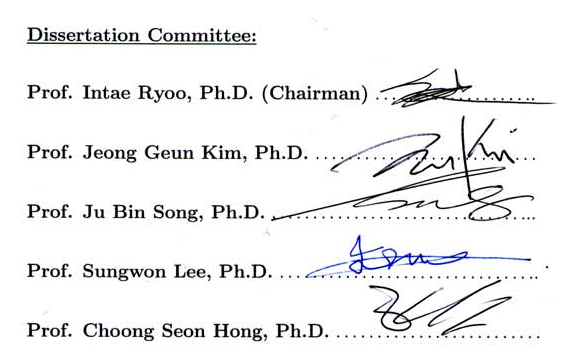
\includegraphics[scale=1.25]{Fig_Thesis_Signature.eps}
%%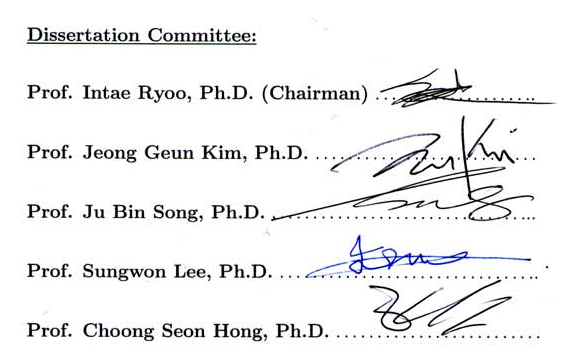
\includegraphics[width=1.62in,height=2.4in]{Fig_Thesis_Signature.eps}
%%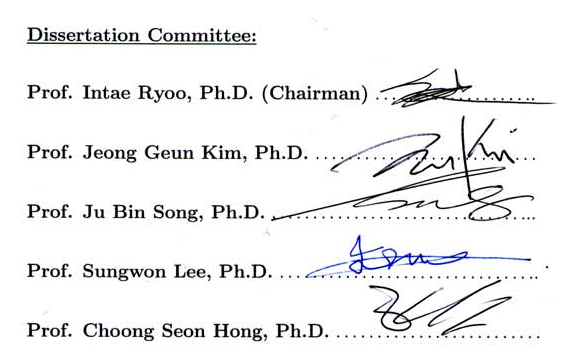
\includegraphics[width=4.5in]{Fig_Thesis_Signature.eps}
%\label{Fig_Thesis_Signature}
%%\end{minipage}
%\end{figure}
%%
\end{center}
\end{titlepage}
\sloppy
%
\titlepage
%

%\begin{titlepage}
\begin{center}
%
%\vspace*{0.5cm}
%
\noindent{\LARGE \textbf{Thesis Approval}}\\
%\vspace*{1.2cm}
%
%\noindent{\LARGE \textbf{{\fontfamily{ptm}\selectfont Path selection and channel access for IEEE 802.11s Wireless Mesh Network}}}\\
%
%\noindent{\LARGE \textbf{{\fontfamily{ptm}\selectfont High performance extensions of IEEE 802.11s standardization for Wireless Mesh Networks}}}\\
%
 Student's Name:\\ 
 Student's ID:\\ 
 Thesis Title: :\\ 


%\noindent{\LARGE \textbf{{\fontfamily{ptm}\selectfont Enhanced channel access and path selection for IEEE 802.11s Wireless Mesh Networks}}}\\
%
\vspace*{.5cm}
We the undersigned, recommend that the thesis completed by the student listed\\ [-5pt]
 above, in partial fulfillment of B.Sc. Engineering degree requirements, be accepted \\[-5pt] 
by the Department of Computer Science and Engineering, Bangabandhu Sheikh \\[-5pt]
 Mujibur Rahman Science and Technology for deposit. 

\vspace*{1.0cm}
\noindent \large \textbf{Supervisor Approval*} \\[15pt]
............................. \\ [-5pt]
Name of Supervisor \\ [-5pt]
Designation of Supervisor \\ [-5pt]


\vspace*{1.0cm}
\noindent \large \textbf{Additional Approvals ( if requires)*} \\[15pt]
  ............................. \\ [-5pt]
  Name of Supervisor \\[-5pt]
  Designation of Supervisor \\[-5pt]

\vspace*{1.0cm}
\noindent \large \textbf{Departmental Approval} \\[15pt]
............................. \\ [-5pt]
Name of Head of the Department \\ [-5pt]
Chairman, Department of Computer Science and Engineering \\ [-5pt]
%
%\vspace*{4.5cm}
%\vspace*{1.75cm}
%\noindent \large \textbf{Supervised by} \\[-7pt]
%\noindent \Large \textbf{Prof. Choong Seon Hong, Ph.D.} \\
\vspace*{1.5cm}
\noindent{\large \textbf{Bangabandhu Sheikh Mujibur Rahman Science and Technology}}\\
\noindent{\large \textbf{University, Gopalganj, Bangladesh}}\\[-15pt]


%
\end{center}
\end{titlepage}
\sloppy
%
\titlepage
%

%\begin{titlepage}
\begin{center}
%
\vspace*{0.5cm}
%
\noindent{\large \textbf{\textcolor{white}{Thesis for the B.Sc Engineering}}}\\
\vspace*{1.2cm}
%
\vspace*{5.5cm}
%
%\noindent \large \emph{\textbf{To my parents and my wife}} \\
\noindent \large \emph{\textbf{Dedicated to my parents, Mr. A  \\
And \\
Mrs. B}} \\
%
\vspace*{4.5cm}
%
\end{center}
\end{titlepage}
\sloppy
%
\titlepage
%


\switchchapter{fake} 
\addcontentsline{toc}{chapter}{Acknowledgment}
%
% -------------------------------------------------------------------- 
%\pagenumbering{roman} \setcounter{page}{1} 
\chapter*{Acknowledgment\markboth{Acknowledgment}{Acknowledgment}} 
%\renewcommand{\baselinestretch}{1.2} 
%

At first I like to thank almighty Allah who gives me ability to perform the Thesis. Then I like to give many thanks to my thesis supervisor Md. Nesarul Hoque, Lecturer, Department of Computer Science and Engineering, who encouraged, supervised and supplied necessary requirements and guideline in performing this work. His inspiration for doing research on Bangla Document Ranking by using Term Frequency and Cosine Similarity let me capable to complete the Thesis. I am grateful to him for his unvarying encouragement and simulating ideas. I also like to give thanks to all my teachers and also that of my friends who gave me advice for the completeness of the thesis. Finally I like to special thank to my parents and all my well wishers for their encouragement and support along my study life.


\vspace{1cm}

\hfill \textbf{Shraboni Afroz Samapti} 

%\hfill December, 2016
%


%
%: ----------------------- abstract ------------------------
%
% Your institution may have specific regulations if you need an abstract and where it is to be placed in the document. The default here is just after title.
%
\frontmatter{}
%
% adding the abstract 
% this also adds the abstract in the table of contents
\fancyhead[RO, RE]{\thepage}
\setcounter{tocdepth}{2}
%
\switchchapter{fake} 
\addcontentsline{toc}{chapter}{Abstract}
%
% Thesis Abstract -----------------------------------------------------
%
% -------------------------------------------------------------------- 
%\pagenumbering{roman} \setcounter{page}{1} 
%\noindent{\large  \textbf{{\fontfamily{ptm}\selectfont Supergraph based Periodic Behavior Mining in Dynamic Networks}}}\\
%by \\
%Sajal Halder  


\chapter*{Abstract\markboth{Abstract}{Abstract}}

Bengali is one of the ten most spoken languages in the world, with almost 200 million speakers. Growing online resources reveal a clear need for Bengali language applications and retrieval systems. The development of the internet, there are huge number of Bangla news articles are published every day on the web from different sources and this amount is growing rapidly day by day. Therefore, people have not enough time to read each document with a specified time limit. Bangla document ranking handles this difficulty with an efficient manner. Although, there are more works have been done in English and other European languages, but there is no contribution are present in bangla language to rank a document.  In our thesis, we rank bangla document using term frequency and cosine similarity. We take document as vector and query as vector. We measure term frequency each word in each document. Then finding out score using cosine similarity. Then sorted the scores and ranked the documents. We demonstrate the effectiveness of the technique for bangla document ranking.


%
% adding the acknowledgment 
% this also adds the acknowledgment in the table of contents

%
%: ----------------------- contents ------------------------
%
\setcounter{secnumdepth}{3} % organisational level that receives a numbers
\setcounter{tocdepth}{3}    % print table of contents for level 3
\switchchapter{fake} 
\renewcommand\contentsname{Table of Contents}
%\addcontentsline{toc}{chapter}{Table of Contents} 
\tableofcontents            % print the table of contents
\cleardoublepage
% levels are: 0 - chapter, 1 - section, 2 - subsection, 3 - subsection
%
%: ----------------------- list of figures ------------------------
\switchchapter{fake} 
%\addcontentsline{toc}{chapter}{List of Figures}
\listoffigures	% print list of figures
\cleardoublepage
%
%: ----------------------- list of tables ------------------------
\switchchapter{fake} 
%\addcontentsline{toc}{chapter}{List of Tables}
\listoftables  % print list of tables
\switchchapter{real}
\newpage
%
%: ----------------------- list of algorithms ------------------------
\switchchapter{fake} 
%\addcontentsline{toc}{chapter}{List of Algorithms}
\listofalgorithms
\switchchapter{real}
%
\mainmatter{}
\fancyhead[RE,LO]{{\thesection}\hspace{0.5em} {\footnotesize\rightmark} }
\renewcommand{\headrulewidth}{0.5pt}
%
% start the arabic page numbering
\pagenumbering{arabic} \setcounter{page}{1} 
%
% now switch to real chapters
%
\chapter{Introduction}
\label{Ch_Chapter1}

\section{Introduction}

In a real retrieval application (e.g.,Web search), the retrieval results using the initial query given by the user may not be satisfactory to the user; often, the user would need to revise the query to improve the retrieval/ranking accuracy. For some information seeking activities, the user may modify his query several times for one information need. In such an interactive retrieval scenario, the information available to us is more than just the current user query and the collection of documents. This paper summaries a set of experiments with term weighting for documents, using the measurement of term importance within an entire document collection. Then taking query it finds the relevant   documents, if it exists then score the documents and sorting the scores it finds out the ranked documents. It is efficient while searching any document suppose in google users write the word or sentence that is called query,my proposed  process will compute the importance of  word and rank the documents sequentially which were in maximum times in documents.

\section{Background and Present State of the Problem}

Bangla document ranking is an important aspect but no such research work had done on bangla language. Various methods and techniques have implied to rank documents of different country of different languages. In reference the importance of a term within the entire document collection has found, then number of term matches between a query and a document , they used two functions 1)the raw frequency and 2)the  log2  of frequency. Then doing normalization for document length they combined the mesures and rank the documents.In reference, they used term frequency and inverse term frequency,they compute the document ranking  performance using precision and recall.In reference, they used MMR method for  ranking documents.
I have mentioned earlier, no research work yet not performed on bangle.  As there are several techniques for document ranking is present, these have their own limitations. One of the big problem of these systems is the accuracy is 	not better. If we need to implement these systems in real time purpose, the accuracy should increase otherwise it will be inefficient. So, I tried to increase the accuracy.

\section{Motivation and Aims}

Today the field of natural language processing(NLP) is increasing. As a nation we have the historical background of  language movement, which reminds us that everyone has the right to communicate using their own language. The growth in electronically available documents makes research and applications in automatic document ranking more and more important. Huge number of available documents in digital media makes it difficult to obtain the necessary information related to the needs of a user. In order to solve this issue, document ranking system can be used. Many work have done in various languages in differnet countries but there is no previous works in bangla on the basis of  document ranking. It encourages me to do the work on bangla document ranking . Now my aim is to identify the document on the basis of  importance of words in bangla so that while doing web search user can see the ranked document corresponding their  given query. By using the ranking process, a user can decide if a document is related to his/her needs without reading whole document.
Document ranking systems can be categorized as extractive or abstractive according to the way the ranking is created. In extractive ranking approaches, the goals are identifying most important concepts in the input and giving relevant documents found in the document set as an output.
In abstractive ranking approaches, first the system understands the texts and then it creates ranking with its own words. The abstractive ranking is similar to the way a person creates ranking. Abstractive ranking remains as a difficult task in natural language processing.


\section{Objectives and Specific aims}

From the above discussion it is found that bangla document ranking is an important thing in our country while reading any bangla documents or newspapers. The objectives of my research are to identify the relevant documents within the given user query.
And the specific aim is to rank relevant document with corresponding query. The query is matched word by word in relevant documents and ranked documents with cosine similarity.

\section{What is NLP \& Document Ranking?}

Natural Language Processing, NLP is a branch of artificial intelligence that deals with analyzing, understanding and generating the languages that humans use naturally in order to interface with computers in both written and spoken contexts using natural human languages instead of computer languages.

\subsection{Document Ranking}

Document ranking is the process of ranking documents with document and query.

\begin{figure*}[htp]
	\centering
		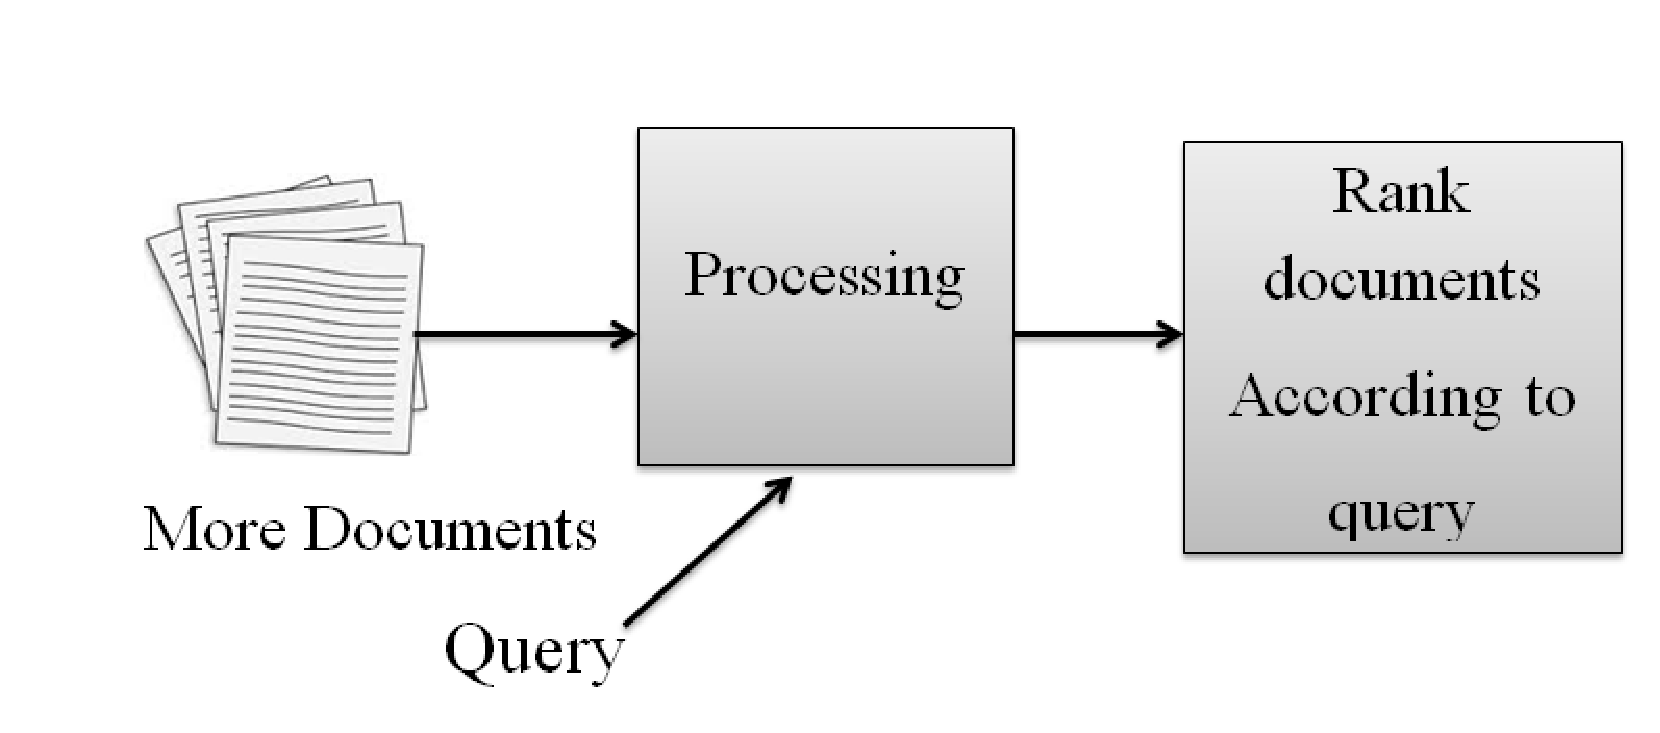
\includegraphics[width=.65\textwidth]{figure/one.eps}
	\caption{Main Process of our system}
	\label{Figure:process}
\end{figure*}





\section{Organization of the Thesis}
%
The dissertation is organized as follows: 

\begin{itemize}

\item {•} \textbf{Chapter 1 Introduction.} In this chapter an introduction to the periodic patterns mining researches is presented. The definition, importance and existing approaches are clearly introduced. After that, the dissertation focuses the contribution. 

\item {•} \textbf{Chapter 2 Related Work.} This chapter first shows the state of the art methods of the periodic patterns mining research. Then describe two existing periodic pattern mining works $PSEMiner$ and $ListMiner$ in dynamic networks. The limitations of these methods are clearly addressed, as these are the focuses of this dissertation. 

\item {•} \textbf{Chapter 3 SPBMiner.} We present our proposed technique for mining periodic behaviors in dynamic networks.  

\item {•} \textbf{Chapter 4 Experiments Analysis.} In this chapter, it has been shown the effectiveness and efficiency of our proposed method.

\item {•} \textbf{Chapter 5 Conclusion and Future Work.} Finally, this chapter concludes the dissertation indicating the limitations and future works.
\end{itemize} 
%

\chapter{Literature Review}
\label{Ch_Chapter2}


Prior to many works has been done by many researchers on English for ranking document. They used many methods or technique for ranking document. There are some overview of previous works that is given below--

\section{Donna Harman,1986}

The use of term weighting in a document produces significant gains in perfonnance, up to a 44\% improvement in average precision over simple matching. Additionally the following conclusions can be drawn from the experiments.

\begin{enumerate}
	\item Here three types of measures tested
	\begin{itemize}
		\item the importance of a term within a document collection
		\item the importance of a term within a given document, and
		\item the length of a document, are all important in term weighting of documents
	\end{itemize}
	
	\item The two types of term-importance factors, impatience within a collection, and importance within a given document, measure term usage in two complementary places-within a given document and within an entire document collection-- and combining them produces a cumulative effect
	
	\item The normalized noise measure of term importance within a document collection is a viable alternative measure to the inverted document frequency measure. Using the log2, of the frequency of a term within a document instead of its raw frequency produces a superior measure of the importance of a term within a given document.
	
	\item Adding the number of matches between a document and a query to a term weight produced by any combination involving a factor that measures term importance within a collection does not produce significant improvement in performance, at least for this test collection and for full word indexing.
	
	\item It is important to consider the length of a document in ranking. Dividing the total term weight by the log of the document length produces significant performance improvement for this test collection.
	
\end{enumerate}


\subsection{Limitation}

The future research is needed to resolve some of the issues. The log2 of the frequency and of the document length is only one possible function of these measures. there is no removal stop words and stemming.

\section{Kent E. Seamons and Dik Lun Lee(1997)}

In this paper they used Vector Space Model for ranking document. They showed five methods for ranking method. They are…

\subsection{Method 1}

The full vector is rarely stored internally as is because it is long and sparse. Instead, document vectors are stored in an inverted file that can return the list of documents containing a given keyword and the accompanying frequency information. Besides, direct comparison between the vectors is slow because it would incur N vector comparisons. Vector comparison can be facilitated with an inverted file as follows.


\begin{algorithm}[H]

\While{every query term q in Q}{

		retrieve the postings list for q from the inverted file\;
		
		\While{each document d indexed in the postings list}{
		
			score(d)=score(d)+tf(d,q)*idf(q)\;
				
		}
}

Normalize scores\;
Sort documents according to normalized scores\;

\caption{Vector Comparison}

\end{algorithm}


With an inverted file, the number of postings lists accessed equals the number of query terms. The computational cost is acceptable for queries of reasonable size. Unfortunately, the computation of the normalization factor is extremely expensive because the term \(\sum_{j=1}^{V}w^2(i,j)\) in the normalization factor requires access to every document term, not just the terms specified in the query. Nor can the normalization factor be precomputed under the \(tf *idf\)  method, because every insertion and deletion on the document collection would change $idf$ and thus the precomputed normalization factors.

\subsection{Method 2}

For this second method, to approximate the effect of normalization we use instead the square root of the number of terms in a document as the normalization factor. While this still favors long documents, the effect of document size is not as significant as it is without any normalization. This normalization factor is much easier to compute than the original one; also, pre computation is possible. With the approximation, the formula becomes\\

\(sim(Q,D_i) = \frac{\sum_{j=1}^{V}w_{Q,j}*w_{i,j}}{\sqrt{number of terms in D_i}}\)

\subsection{Method 3}

This method lets us further simplify the computation by simply dropping the normalization factor:\\

\(sim(Q,D_i) = \sum_{j=1}^{V}w_{Q,j}*w_{i,j}\)\\

That is, the document score equals the inner product of the document and query vectors. Instead of computing the angle between the document and query vectors, this formula computes the length of the projection of the document. vector onto the query vector. It is quite clear that the document score is directly proportional to the length of the document vector.

\subsection{Method 4}

This method only makes use of term frequencies in the calculation and ignores $idf$. It simplifies the computation as well as saving the file structure needed for storing the $df$ values.\\

\(sim(Q,D_i) = \sum_{j=1}^{V}w_{Q,j}*tf_{i,j}\)

\subsection{Method 5}

This method ignores the term frequency $(tf)$ information but retains the $idf$ values in determining term weights:\\

\(sim(Q,D_i) = \sum_{j=1}^{V}w_{Q,j}*w_{i,j}\) , where 
\[ w_{Q,j} =
  \begin{cases}
    1       & \quad  j \in Q \\
    0  & \quad \text{Otherwise } \\
  \end{cases}
\]

and

\[ w_{i,j} =
  \begin{cases}
    1       & \quad  j \in D_i \\
    0  & \quad \text{Otherwise } \\
  \end{cases}
\]\\

The $idf$ values have the same effect as before. That is, they diminish the significance of words that appear in a large number of documents.


\subsection{Method 6}

This method is the simplest in the family. It ignores both $tf$ and $idf$ values and therefore measures the number of common terms in the document and query vectors.\\

\(sim(Q,D_i) = \sum_{j=1}^{V}w_{Q,j}*w_{i,j}\) , where 
\[ w_{Q,j} =
  \begin{cases}
    1       & \quad  j \in Q \\
    0  & \quad \text{Otherwise } \\
  \end{cases}
\]

and

\[ w_{i,j} =
  \begin{cases}
    idf_i       & \quad  j \in D_i \\
    0  & \quad \text{Otherwise } \\
  \end{cases}
\]\\

The performance gain is as much as 25 percent over baseline. However, there is no overwhelming evidence to indicate which combination works best. For concept queries, we find it best to use only inverse document frequencies while ignoring term frequencies, but for natural-language queries both frequencies are needed— ignoring either one will produce poor results. Furthermore, the approximate normalization factor we suggest here gives the best performance and is computationally efficient. They have found that high-frequency terms or terms in the neighborhood of hits selected from context units containing at least one hit give the best feedback performance. In some cases, the gain in average precision is as much as 20–25 percent. On the other hand, although the data shows slight improvement in using terms around hits overhigh-frequency terms, the evidence is not overwhelming. To develop an efficient and effective retrieval system, many implementation issues must be considered.



\section{Xuehua Shen \& ChengXiang Zhai (2003)}

In interactive information retrieval \cite{shen2003exploiting}, at any moment, they  may assume that a sequence of “past queries”, or “query history”, q1……qk-1, are available for a topic, and the current user query is qk. Normally, only qk is used to rank the documents in the collection. They proposed to combine q1, ..., qk-1 together with qk to have a richer model of the user’s information need. Our basic retrieval model is the KL-divergence retrieval model. 
They explore two different strategies –combining query results and combining query models. Combining query results means that we merge the results from q1, ..., qk by taking an average of the rank of each document. Such a method would reward a document that has been ranked high by all the queries. Combining query models means that we estimate a query language model for each query qi using the maximum likelihood estimator, and then take an average of these query models to obtain a contextbased query model, which is then used to rank documents with the KL-divergence ranking formula.
The probability of a word w according to the context-based query model is given by\\


\(p(w|q1,……q^k) = \frac{1}{k}\sum_{i=1}^{k}\frac{c(w,q^i)}{|q^i|}\)\\

where, $c(w; qi)$ is the counts of word w in query $qi$ and $|qi|$ is the length of query $qi$. Note that this is different from concatenating the query text of $q1, ..., qk$ to obtain a long query, since they normalize the counts of a query word by the length of each query, which can avoid dominance of one single query. For each document d, they also estimate a smoothed document language model using the Dirichlet prior smoothing method. We then rank documents by the KL divergence value of the query model and the document model. That is, document $d$ has a score of\\

\(\sum{p(\frac{w}{q1},........q^k)log(1+\frac{c(w,d)}{\mu p(W|C)})}+log\frac{\mu}{\mu +d}\)\\

where, $p(w|C)$ is the collection language model and $µ$ is the Dirichlet prior smoothing parameter . In interactive information retrieval, especially for hard topics, the user would generally need to submit a sequence of queries to the search system. They demonstrate that using query history to expand the current query can consistently improve the retrieval performance. 

We have only explored the most basic methods for exploiting the query history; more sophisticated analysis is certainly possible and interesting to explore (e.g., term sequence analysis and unequal weighting of different queries).


\section{Our Proposed System}

We use term frequency and cosine similarity for ranking bangla multiple document. For finding cosine similarity we use the equation\\

\(\cos(q,d) = \frac{\overrightarrow{q}.\overrightarrow{d}}{|\overrightarrow{q}||\overrightarrow{d}|}\)\\

We take query as a vector and document as a vector then find similarity between them and calculating scores we rank document.








\chapter{Proposed System}
\label{Ch_Chapter3}


We have used two methods for ranking document. One is term frequency and another is cosine similarity.

\section{Creating Document Vector}
The process of creating document vector is given below.

\subsection{Term Frequency}

A term that appears many times within a document is likely to be more important than a term that appears only once.\\
D1: {\unicodefont আমি  বাংলাদেশকে ভালবাসি । বাংলাদেশ নদীমাতৃক দেশ।}  \\ 
D2: {\unicodefont আমি বাংলাদেশের নাগরিক । কিন্তু বাংলাদেশের সকল  নাগরিক তাদের মোলিক অধিকার পায় না।} \\
D3: {\unicodefont বাংলাদেশ উন্নয়নশীল দেশ। এখনো উন্নয়নের দিক থেকে পিছিয়ে আছে বাংলাদেশ । } \\

After performing the term frequency calculation we get the table \ref{tab:tab1}. Which is showing the value each word each document.

\begin{table*}[htp]	
\centering

  \caption{Parameters of datasets }
\vspace{0.5cm}
\begin{tabular}{|c|c|c|c|} 
\hline

Term & 	Doc1 & Doc2 & Doc3  \\ \hline
{\unicodefont আমি} 		& 1 & 1 &	   \\ \hline
{\unicodefont বাংলাদেশ}	& 2 & 2 & 2   \\ \hline
{\unicodefont ভালবাসি }	& 1 &  &   \\ \hline
{\unicodefont উন্নয়নশীল } 	&  &  &   \\ \hline
{\unicodefont দেশ } 	&  &  & 1  \\ \hline
{\unicodefont নদীমাতৃক }  & 1 &  &   \\ \hline
{\unicodefont কিন্তু}	&  & 2 &   \\ \hline
{\unicodefont সকল}সকল	&  & 1 &   \\ \hline
{\unicodefont মোলিক}	&  & 1 &   \\ \hline
{\unicodefont অধিকার}	&  & 1 &   \\ \hline
{\unicodefont পায়}	&  & 1 &   \\ \hline
{\unicodefont এখনো}	&  &  & 1  \\ \hline
{\unicodefont দিক}  &  &  & 1 \\ \hline
{\unicodefont থেকে} &  &  & 1 \\ \hline
{\unicodefont পিছিয়ে}&  &  & 1 \\ \hline
{\unicodefont আছে}&  &  & 1 \\ \hline
{\unicodefont নাগরিক}&  & 2 &  \\ \hline
{\unicodefont না} &  & 1 &  \\ \hline
{\unicodefont তাদের}&  & 1 &  \\ \hline

\end{tabular}
\label{tab:tab1}
\end{table*}



\subsection{Stop Word Removing}
Documents contain words that do not add information but are necessary for syntactical formation,such as words like {\unicodefont এবং , অথবা , কিন্তু } etc. Since these words are less useful and less informative,  they introduce  noise into the document representation. In order to get rid of these kind of words, a stop word removal step is used.  Stop word removal is done using predefined, human-made list of words. Since a predefined list is used, this approach is language dependent. Instead of using these kinds of lists, a frequency threshold can be used. If a word is seen more\/less frequently than predefined threshold, that word can be considered as stop word. But decision of threshold is another issue to be considered.

\subsection{Stemming}

In a document a word can be seen in different formats, such as plural vs. singular, present vs. past tense, etc. Most of the time these words have the same meaning and treating them differently is unnecessary. In order to use these words as the same token(concept), stemmers are used.
Stremmers are tools that reduce the orginal word forms into roots(stems) of these words. Stemmers are necessary to represent different forms in a single format and to reduce memory usage for storing the words. Also, smaller list of words make it easir to perform calculations. As a result of performing stemming,document representation is less noisy and more dense. The efficiency of a stemmer is important while performing further calculations. In Figure \ref{Figure:stemm} ,we can see the full process of ranking.

Sometimes stemmers can do over-stemming such that two words are given the same stem,while it should not be. For example, the words {\unicodefont “বাংলাদেশের”} and {\unicodefont “বাংলাদেশকে”} are two different words, which should not be stemmed into the same root. But stemmers can find out their root as {\unicodefont “বাংলাদেশ”}. Another steamming problem is related to under stemming such that two words should have been stemmed into the same word, but have not been. for example, {\unicodefont “হাসি”} and {\unicodefont ‘হাসানো’} can be found as two different stems,instead of one.



\subsection{Weighting Term}

Then find weight in a document for each term using the equation \ref{eq:eq1}

\begin{equation}
Weight++=postings[term][doc]*IDF
\label{eq:eq1}
\end{equation}

%\(Weight++=postings[term][doc]*IDF\)

Then assigning document IDS we keep them into database as vector after doing following steps which is shown in Figure \ref{Figure:indexing}.

\subsubsection{Inverse Document Frequency(IDF)}

A term that occurs in a few documents is likely to be a better discriminator than a term that appears in most or all documents.

Then assigning document IDS we keep them into database as vector after doing these steps.


\begin{figure*}[htp]
	\centering
		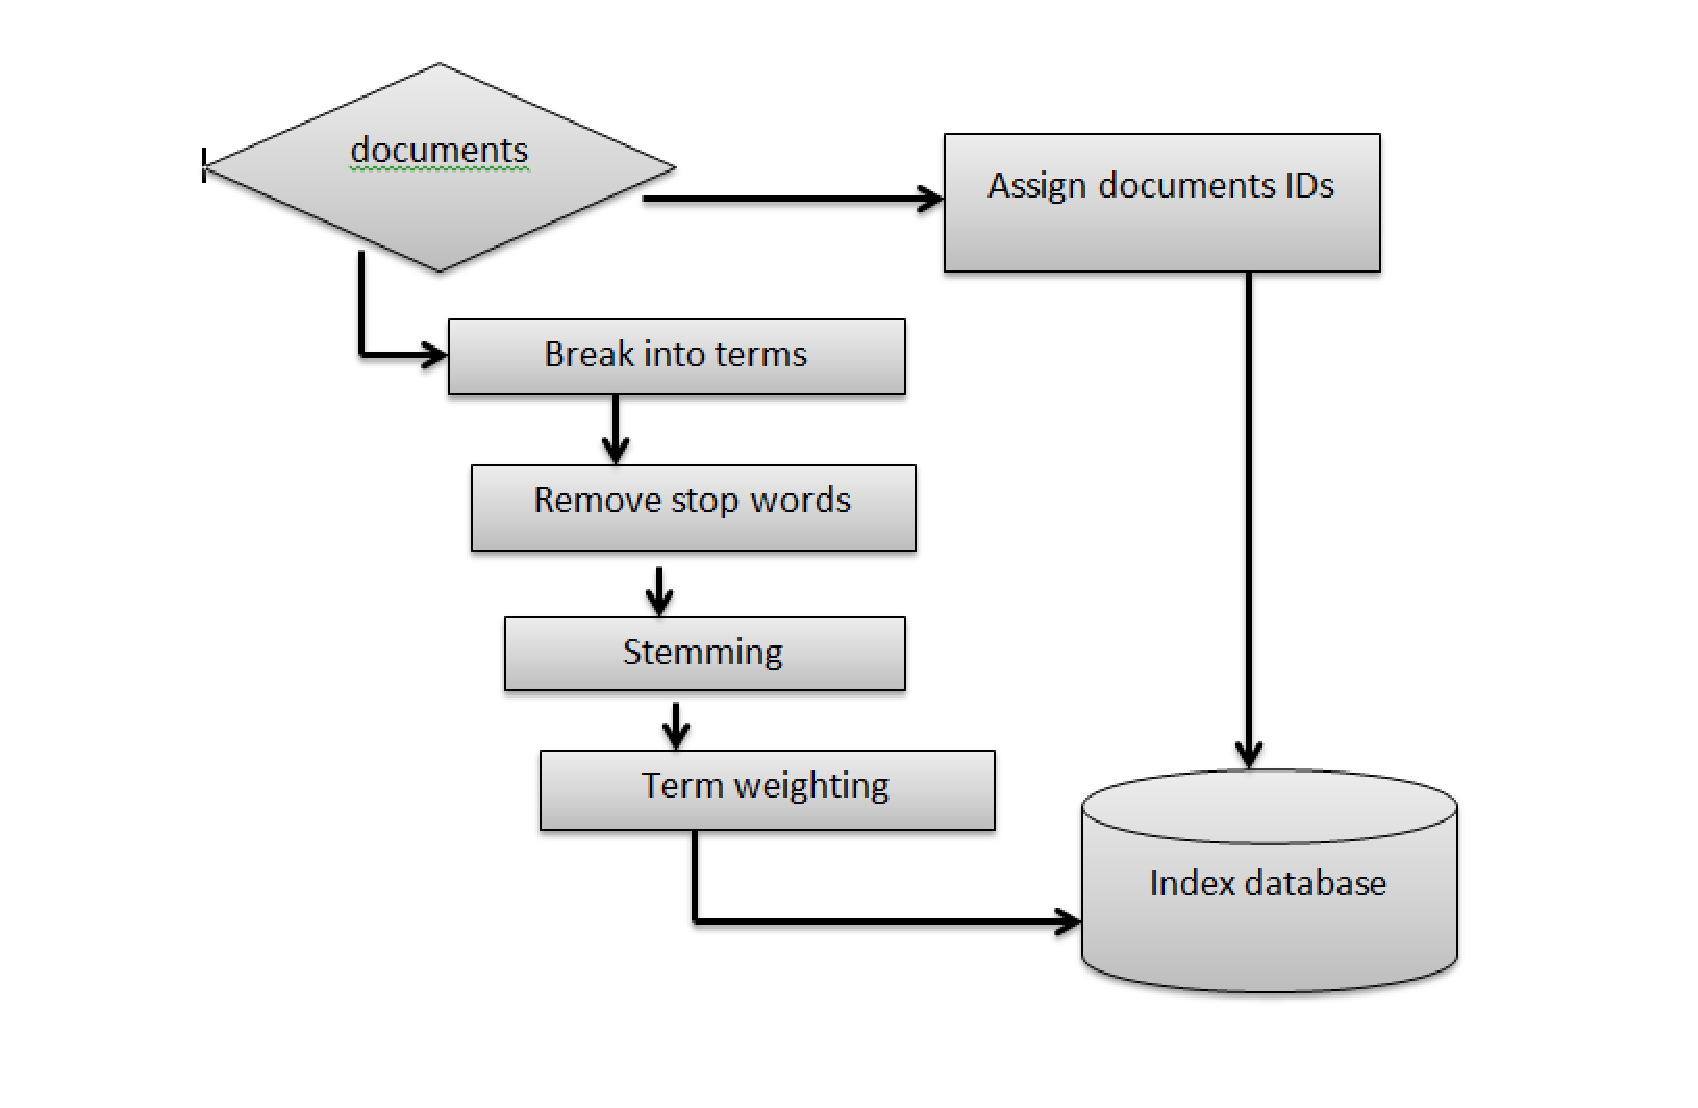
\includegraphics[width=.65\textwidth]{figure/two.eps}
	\caption{\textbf{Indexing Document Ids \& keep it in a vector.}}
	\label{Figure:indexing}
\end{figure*}


\section{Preprocessing of Taking Query}

For taking search query the preprocessing steps have to be done. After taking query step by step process has been done . And then match query with relevent documents. The preprocessing steps are showing in the figure \ref{Figure:inquery} below.


\begin{figure*}[htp]
	\centering
		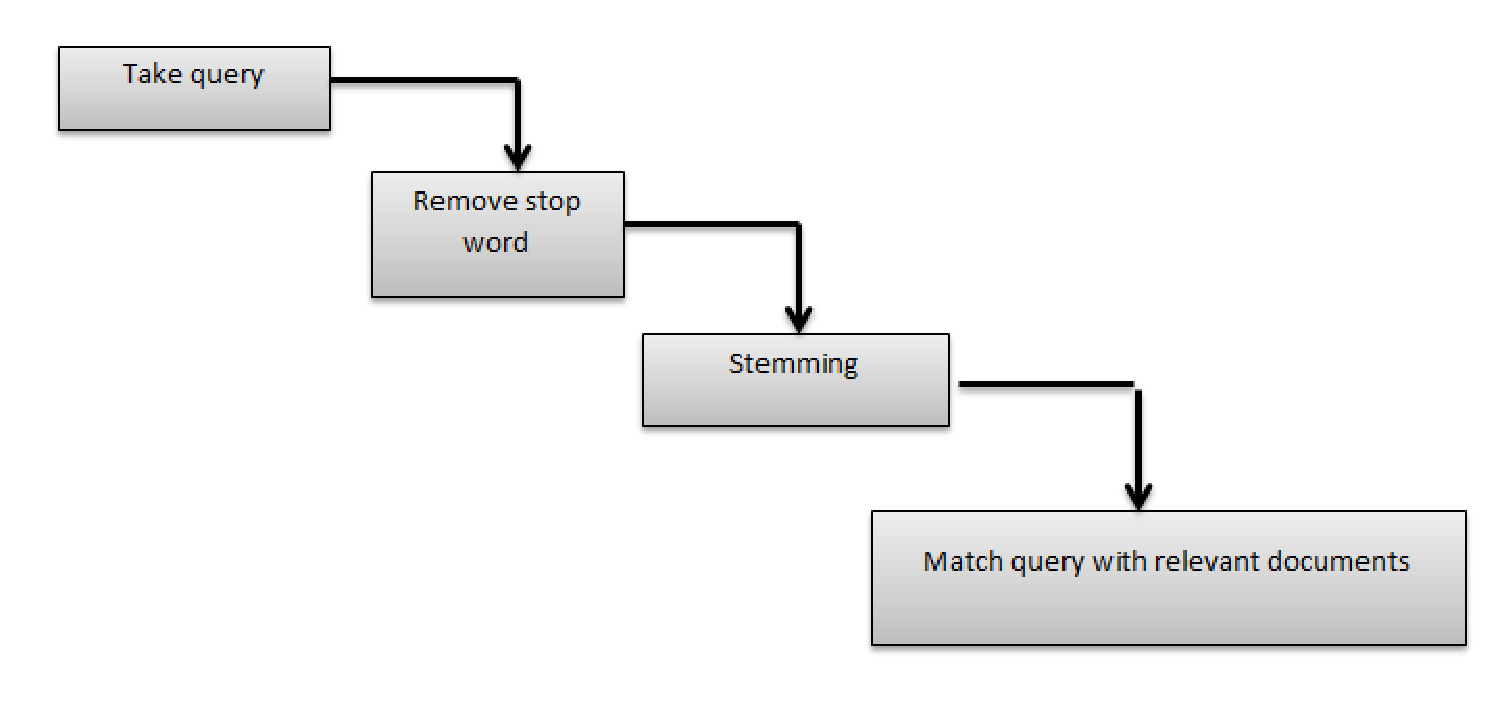
\includegraphics[width=.65\textwidth]{figure/three.eps}
	\caption{\textbf{Pre processing of Input query}}
	\label{Figure:inquery}
\end{figure*}


\subsection{Removal of Stop Word}

The less importance word should be removed from query. Sometimes input query contain words that do not add information, such type words {\unicodefont ‘এবং’ , ‘অথবা’ , ‘কিন্তু ’} etc should remove from document.

\subsection{Stemming}

Finding root words from other similar words which have the same meaning and treating them differently is unnecessary. Figure \ref{Figure:stemm} showing the process.

\begin{figure*}[htp]
	\centering
		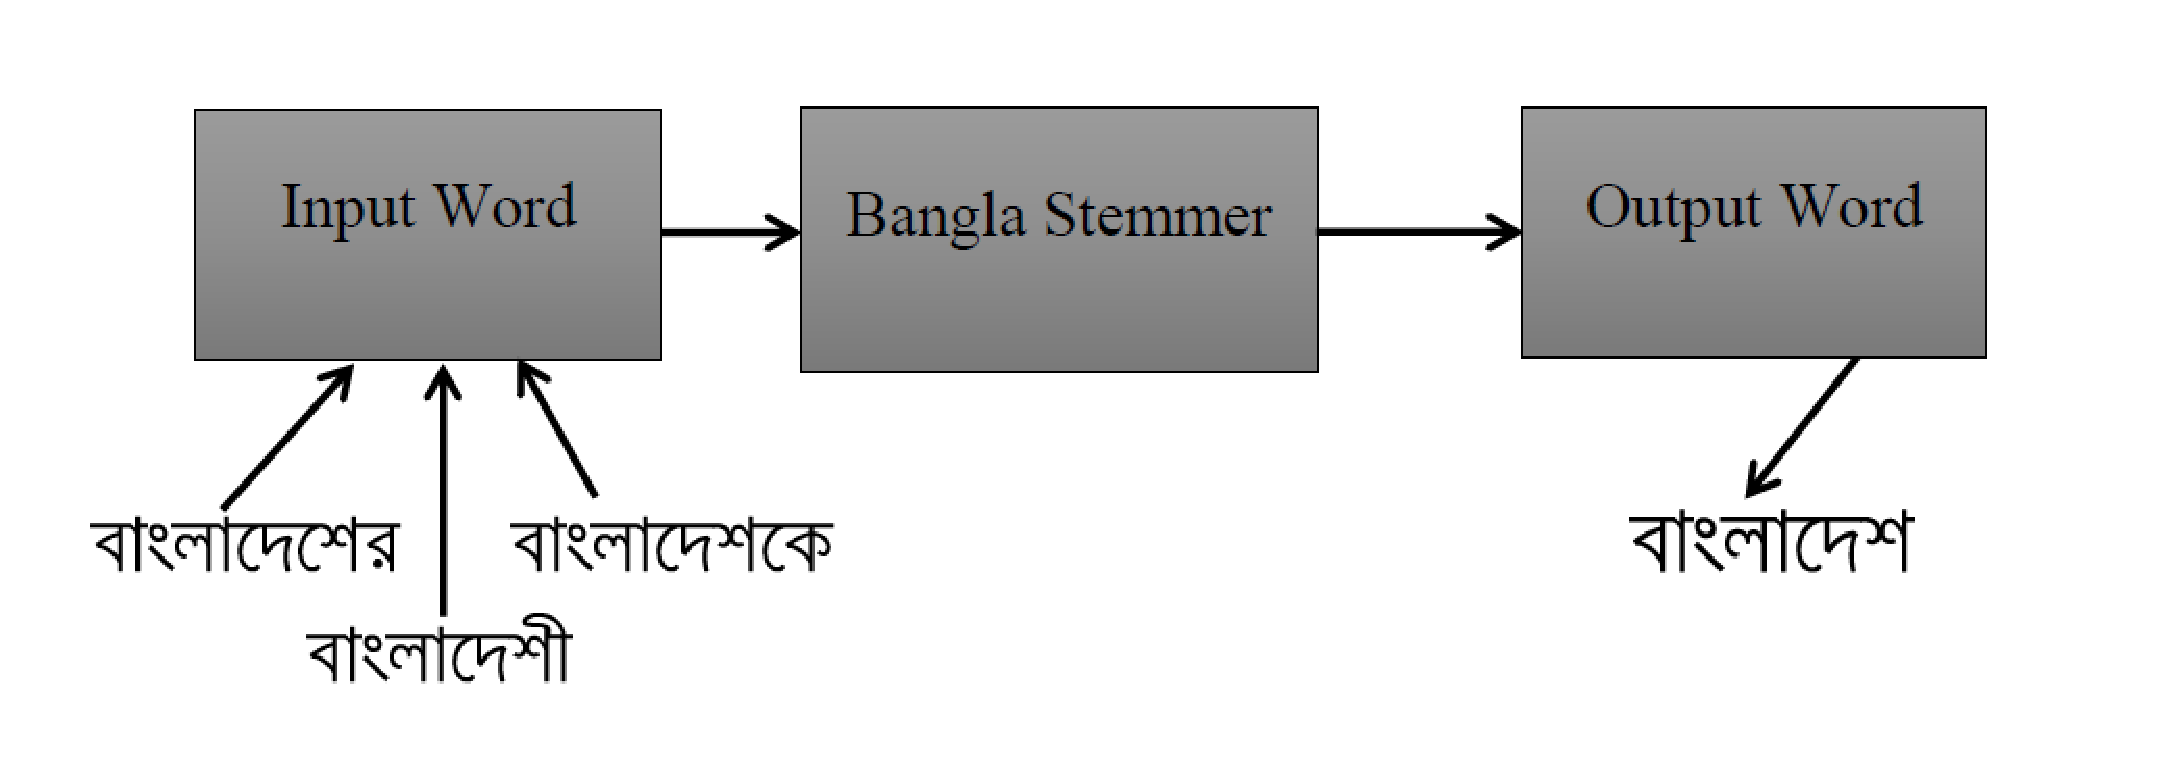
\includegraphics[width=.65\textwidth]{figure/four.eps}
	\caption{\textbf{Stemming processing}}
	\label{Figure:stemm}
\end{figure*}


\section{Cosine Similarity}

The query matches with relevent documents. If exists, find out the relevent documents and give them a scores using query term’s IDF multiplying with weight. Then sort the values and rank the documents.

Example:
There are three documents.\\
	D1: {\unicodefont আমি  বাংলাদেশকে ভালবাসি । বাংলাদেশ নদীমাতৃক দেশ।} \\
	D2: {\unicodefont আমি বাংলাদেশের নাগরিক । কিন্তু বাংলাদেশের সকল  নাগরিক তাদের মোলিক অধিকার পায় না। }\\
	D3: {\unicodefont বাংলাদেশ উন্নয়নশীল দেশ। এখনো উন্নয়নের দিক থেকে পিছিয়ে আছে বাংলাদেশ ।  }\\
	
	%{\unicodefont বাংলাদেশের নাগরিক হিসেবে বাংলাদেশের উন্নতি চাই।}
Input Query: {\unicodefont বাংলাদেশের নাগরিক হিসেবে বাংলাদেশের উন্নতি চাই।}\\

\(Cosine(document , query)  = (document . query) / |document vt | |query vt|\)\\


Now in table \ref{tab:Scoring} we can see the scores after doing the all process.

\begin{table*}[htp]	
\centering

\caption{Scoring Each Document  }
\vspace{0.5cm}
\begin{tabular}{|c|c|c|} 
\hline

	Document Id & Documents & Scores \\ \hline
 1 & D1 &	0.145   \\ \hline
 2 & D2 & 0.543   \\ \hline
 3 & D3  &0.345   \\ \hline


\end{tabular}
\label{tab:Scoring}
\end{table*}

After sorting scores, we get the ranked documents and we can see that in table \ref{tab:Rank}.


\begin{table*}[htp]	
\centering
\caption{Rank Documents  }
\vspace{0.5cm}
\begin{tabular}{|c|c|c|} 
\hline

Document Id & Documents & Scores \\ \hline
 2 & D2 &	0.543   \\ \hline
 3 & D3 & 0.345   \\ \hline
 1 & D1 &0.145  \\ \hline


\end{tabular}
\label{tab:Rank}
\end{table*}


\section{Main Approaches}

When the preprocessing is completed, then our main process focuses on the analysis of the processed output by our own developed tools for Bangla document ranking. Our main approach are includes to generating term frequency vector, assigning cosine similarity to the corresponding document are known as document scoring. Then sorting the scores, we rank the documents. In figure \ref{Figure:graphical} shows the overall graphical view of our proposed system.

\begin{figure*}[htp]
	\centering
		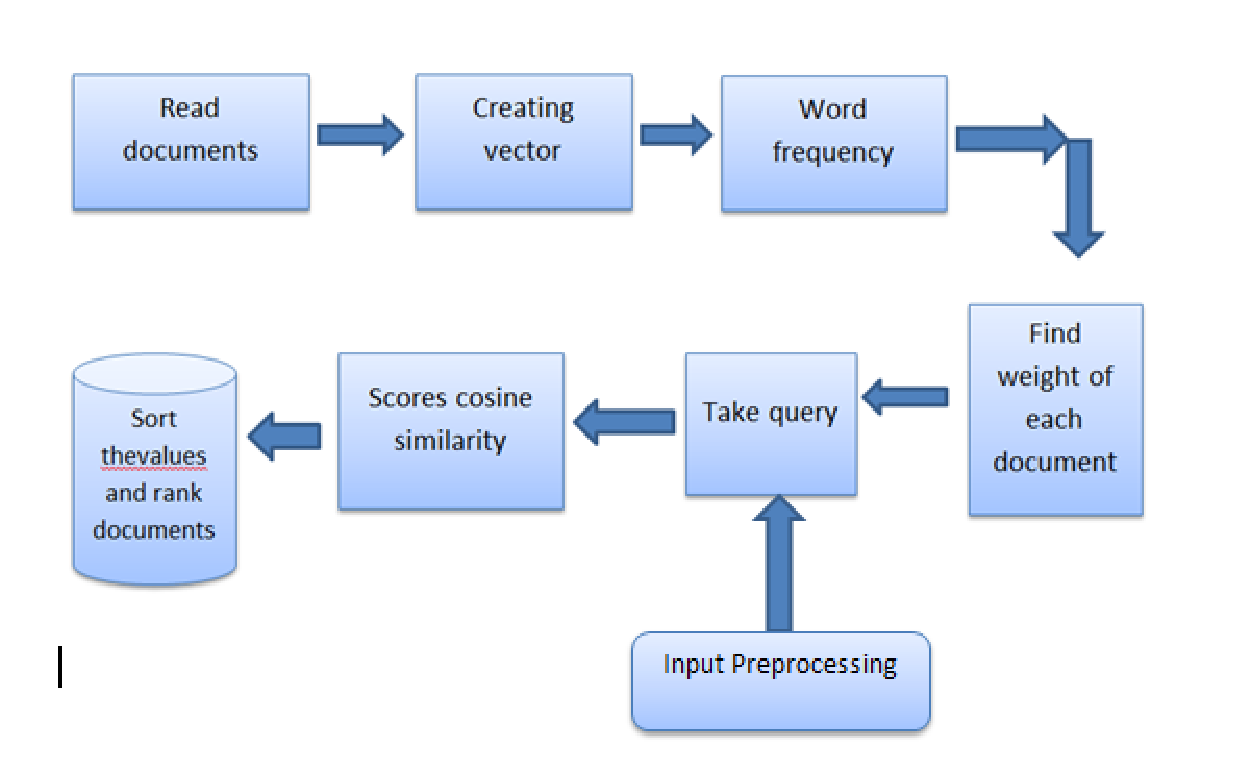
\includegraphics[width=.65\textwidth]{figure/five.eps}
	\caption{\textbf{Overall graphical view of our proposed system}}
	\label{Figure:graphical}
\end{figure*}


\chapter{Experimental Evaluation}
\label{Ch_Chapter4}

\chapter{Experimental Result \& Discussion}
\label{Ch_Chapter5}


\section{Experimental Result}

To examine our ranking, we collect 30 bangla documents from the bangla daily newspaper eg Prothom alo, kaler kontho etc. The documents are written and saved in the text files using UTF-8 format. For each document in our corpus, we consider only one human ranking for evaluation. Evaluation of a system produced ranking is done by comparing it to the human ranking. There are some documents here on boimela.\\

Doc 1 : boimela txt.\\
কলকাতায় বাংলাদেশ বইমেলা থাকছে ৫০ প্রকাশনী । বইয়ের বন্ধুত্ব সীমানা ছাড়িয়ে- স্লোগানে ১ সেপ্টেম্বর থেকে কলকাতায় শুরু হচ্ছে ১০ দিনব্যাপী ‘বাংলাদেশ বইমেলা’। সচিবালয়ে সোমবার সংস্কৃতি সচিব আকতারী মমতাজ এক সংবাদ সম্মেলনে জানান, ষষ্ঠবারের মতো আয়োজিত মেলায় বাংলাদেশের ৫০টি প্রকাশনা প্রতিষ্ঠান অংশ নেবে। ১ সেপ্টেম্বর বিকেল ৫টায় মেলার উদ্বোধন করবেন ইমেরিটাস অধ্যাপক আনিসুজ্জামান। উদ্বোধনী অনুষ্ঠানে থাকবেন পশ্চিমবঙ্গ সরকারের শিক্ষামন্ত্রী পার্থ চট্টোপাধ্যায় ও কবি-প্রাবন্ধিক শঙ্খ ঘোষ। প্রতিদিন দুপুর ২টা থেকে রাত ৮টা পর্যন্ত মেলা উন্মুক্ত থাকবে। শনি ও রোববার বিকাল ৩টা থেকে রাত ৮টা পর্যন্ত মেলা চলবে।
জাতীয় গ্রন্থকেন্দ্র ও রপ্তানী উন্নয়ন ব্যুরোর সহযোগিতায় এবং কলকাতায় বাংলাদেশ উপ-দূতাবাসের ব্যবস্থাপনায় বাংলাদেশ জ্ঞান ও সৃজনশীল প্রকাশক সমিতি গত পাঁচ বছর ধরে কলকাতায় বাংলাদেশ বইমেলার আয়োজন করছে।প্রথম তিন বছর মেলাটি গণকেন্দ্র শিল্প সংগ্রহশালায় হলেও গত দুই বছর ধরে রবীন্দ্র সদনের উন্মুক্ত প্রাঙ্গণে হয়। এবারও এই উন্মুক্ত প্রাঙ্গণে বাংলাদেশ বইমেলা বলে জানান আকতারী মমতাজ।

Doc 2: accident.txt\\
ট্রেনের ধাক্কায় রাবি শিক্ষার্থীর মৃত্যু। ফোনে কথা বলার সময় পেছন থেকে ট্রেনের ধাক্কায় রাজশাহী বিশ্ববিদ্যালয়ের এক ছাত্রীর মৃত্যু হয়েছে। রোববার বিকাল সোয়া ৪টার দিকে বিশ্ববিদ্যালয়ের চারুকলা গেটের কাছে পদ্মা এক্সপ্রেস ট্রেনের ধাক্কায় শান্তনা বসাক মারা যান।  শান্তনা সমাজকর্ম বিভাগের তৃতীয় বর্ষের শিক্ষার্থী। তিনি সিরাজগঞ্জের তাড়াশ উপজেলার মাধইনগর গ্রামের নরেন্দ্রনাথ বসাকের মেয়ে। বেগম রোকেয় হলের আবাসিক শিক্ষার্থী ছিলেন তিনি। প্রত্যক্ষদর্শীরা জানান, শান্তনা বসাক বিশ্ববিদ্যালয়ের চারুকলা অনুষদের পাশের রেল লাইনে হেঁটে হেঁটে মোবাইল ফোনে কথা বলছিলেন। কানে হেডফোন লাগানো ছিল। চারুকলা গেটে দায়িত্বরত পুলিশ সদস্যরা বেশ কয়েকবার তাকে রেল লাইন থেকে সরে যেতে বললেও তিনি খেয়াল করেননি।   ওই সময় রাজশাহী থেকে ঢাকাগামী পদ্মা এক্সপ্রেস ট্রেনটি চারুকলা গেট অতিক্রম করছিল। পেছন থেকে আসা ট্রেনটি থেকে বারবার হর্ন বাজালেও ফোনালাপে মগ্ন থাকায় শান্তনা সরেননি। এ সময় পেছন থেকে ট্রেনটি ধাক্কা মারলে শান্তনা গুরুতর আহত হন। পরে শিক্ষার্থীরা তাকে উদ্ধার করে রাজশাহী মেডিকেল কলেজ হাসপাতালে নিয়ে যান।


Doc 3: rajshahi.txt\\
রাজশাহী মেডিকেল কলেজ হাসপাতালে কর্তব্যরত সহকারী উপপরিদর্শক মো. শফিক বলেন, অতিরিক্ত রক্তক্ষরণের কারণে চিকিৎসা শুরুর আগেই তার মৃত্যু হয়েছে।  বিশ্ববিদ্যালয়ের সমাজকর্ম বিভাগের সভাপতি অধ্যাপক ছাদিকুল আরেফিন বলেন, পরিবারের সদস্যদের খবর দেওয়া হয়েছে। তার ভাই মরদেহ নিতে আসছেন বলে জানিয়েছেন। ময়না তদন্তের পর পরিবারের কাছে মরদেহ হস্তান্তর করা হবে। “বিভাগের তৃতীয় বর্ষের ওই শিক্ষার্থীর অকাল মৃত্যুতে আমরা গভীরভাবে শোকাহত।” নগরীর মতিহার থানার ওসি হুমায়ুন কবির বলেন, “বিশ্ববিদ্যালয়ের এক ছাত্রী ট্রেনে কাটা পড়ে মারা গেছে বলে শুনেছি। তবে এটা আত্মহত্যা নাকি দুর্ঘটনা এ ব্যাপারে নিশ্চিত হওয়া যায়নি। বিষয়টি খোঁজ নেওয়া হচ্ছে।”


Input Query : রাজশাহী বিশ্ববিদ্যালয়ের এক ছাত্রীর মৃত্যু হয়েছে\\

When we apply the proposed system to our bangla document,this machine generate cosine similarity to corresponding query and documents. Finally, the cosine values of coresspondibg documents are given in table 3. The goal 0f document ranking is to present the relevant documents corresponding users query. This process is slightly similar to text summarization. It helps us to find out the documents easily that users want.

When the cosine similarity is enlisted for the corresponding documents then the document is rearranging according to their root document. Finally taking the top rated document is taken for ranking. The ranked document is:\\
		$Accident.txt > Rajshahi.txt > Boimela.text$
		
We balanced Our system to rank with the human ranking, calculating the following scores. For document ranking we let  “Kh”  be the length of human ranking. “Km” the length of the system generated ranking and  “r” the number of ranking they share in major. We defined precision (P), recall (R) and accuracy to compare the two summaries by:\\
\(P =  r/kh \%\)\\
\(R =  r/km \%\)\\
\(Accuracy =  2*r / kh + km \%\)\\


To evaluate the accuracy of our proposed system we examined the 30 documents with the above accuracy equation (3). For this we calculate the precision and recall value using  the above equation  (1) and  (2) sequentially. The output of the given equation are the  input of the proposed system to find the level of accuracy using equation (3). Finally the average accuracy of Bangla document ranking is 88.10\% corresponding with human generated ranking . The accuracy on the basis of equation (3) is given Table      



Finally the average result is around 88.10% .
The graph of the document ranking is


\begin{figure*}[htp]
	\centering
		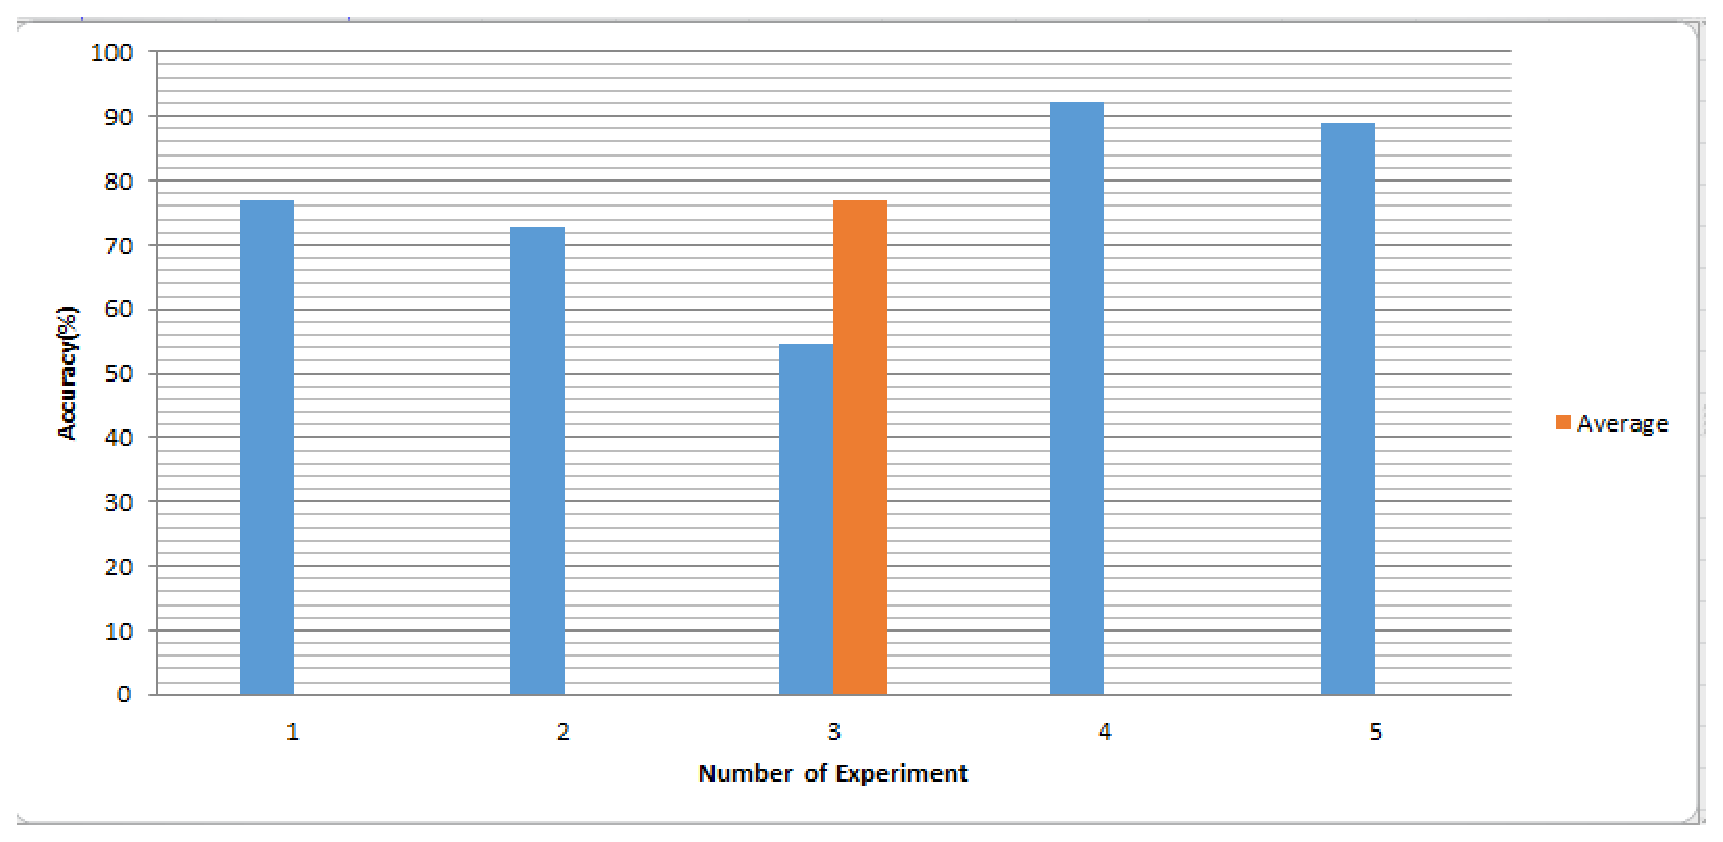
\includegraphics[width=.65\textwidth]{figure/six.eps}
	\caption{Graphical view of document ranking}
	\label{Figure:granking}
\end{figure*}


It is very difficult to determine if a ranking is good or bad. The ranking examined methods can be broadly categorized as human evaluation methods and automatic(machine-based) evaluation methods. A human evaluation is done by comparing system-generated ranking with reference model ranking by human judges.

The main problems with human evaluation are:

\begin{itemize}
	\item The evaluation process is exhausting
	\item It sustains from the lack of unity
\end{itemize}

Two human judges may not agree on each other’s judgements. Since automatic evaluation is performed by a machine, it follows a fixed logic and always produces the same result on a given ranking. Since automatic evaluation process are free from human bias, it provides a consistent way of comparing the various ranking systems.


\section{Discussion}

In this thesis, we explain the basic ideas of hoe to rank different documents according to their relevance. The ideas used are very beautiful. They are some fearsome-sounding vector space model for documents. Instead of thinking of documents and queries as strings or letters, we adopt a point of view in which both documents and queries are represented as vectors in a vector space. In this point of view, the problem of determining how relevant a document is to a query is just a question of determining how parallel the query vector and the document vector are. The more parallel the vectors, the more relevant the document is.

This geometric way of treating documents turns out to be very powerful. It’s used by most modern web search engines, including (most likely) web search engines such as Google as well as search libraries. The ideas can also be used well beyond search, for problems such as document classification, and for finding clusters of related documents.


\chapter{Conclusions and Future Work}
\label{Ch_Conclusion}

\section{Conclusion}

In Bangla document ranking, the term frequency and cosine similarity perform the utmost level of accuracy (88.10\%) than any other existing methods. The model we have described treats all documents on an equal footing. In addition to, this is the extraction based ranking system, is not real time ranking formation. In the typical web search setting it is important to users that the most relevant documents are top-ranked given the large number of potentially relevant documents. For each term in the dictionary, it’s straightforward to pre compute the top 1,000(say) documents for that term. Then for a given multi-term query it’s pretty likely that the top search results will come from one of the pre-computed lists of top documents for the terms in the query.

\section{Future Work}

The problem is that it computes the cosine similarity for every single document in the corpus. In future, ideas that are used in other methods, will be used together with the proposed approaches to improve the performance of the ranking system.

%
\fancyhead[RE,LO]{{\footnotesize\rightmark} }


\renewcommand{\headrulewidth}{0.5pt}
%
\bibliographystyle{IEEEtran}
\switchchapter{fake} 
\addcontentsline{toc}{chapter}{Reference}
\bibliography{reference}
%\bibliography{BibTex}
%
\fancyhead[RE,LO]{{\footnotesize\rightmark} }
\renewcommand{\headrulewidth}{0.5pt}
%
\appendix 
\titlecontents{chapter}[6pc] 
  {\bfseries} 
  {\contentslabel[\appendixname\ \thecontentslabel]{6pc}} 
  {}{\hfill\contentspage} 
%
%\include{Acronyms}
%\include{Notations}
%\fancyhead[RE,LO]{\footnotesize{LIST OF PUBLICATIONS} \hspace{0.5em} {\footnotesize\rightmark} }
\renewcommand{\headrulewidth}{0.5pt}
%
\chapter{List of Publications}
\begin{center}
\textbf{\Large \underline {International Journal Papers}} \\
\end{center}
\begin{enumerate}
%
%\item \textbf{Sajal Halder} and Young-Koo Lee. \textit{Supergrpah based Periodic Behaviors Mining in Dynamic Networks}. In submission.

\item  \textbf{Sajal Halder}, Yongkoo Han, A. M. Jehad Sarkar and Young-Koo Lee. \textit{An Entertainment Recommendation System using the Dynamics of User Behavior over Time}. Decision in process in the Journal of Systems and Software.

\item	Md. Rezaul Karim, \textbf{Sajal Halder} , Byeong-Soo Jeong, and Ho-Jin Choi. \textit{Efficient Mining Frequently Correlated, Associated-correlated and Independent Patterns Synchronously by Removing Null Transactions}. Human Centric Technology and Service in Smart Space, pages 93-103, 2012. 

%\vspace{0.1in}
\item \textbf{Sajal Halder}, A. M. Jehad Sarkar and Young-Koo Lee. \textit{A synthetic trajectory-based moving objects generator}. Under review  in International Journal of Artificial Intelligence Tools.

\item \textbf{Sajal Halder}, Md. Mostofa Kamal Rasel, Yongkoo Han, and Young-Koo Lee. \textit{Mining Spatiotemporal Moving Objects Swarm}. Under review in Kyung Hee University Journal..

\pagebreak


%
\begin{center}
\textbf{\Large \underline{International Conference Papers}} 
\end{center}

\item Sajal Halder, Yongkoo Han and Young-Koo Lee. \textit{Discovering Periodic Patterns using Supergraph in Dynamic Networks}. Accepted in 5th International Conference on Data Mining and Intelligent Information Technology Applications (ICMIA),Jun 18-20, South Korea, 2013.

%
\item Sajal Halder, A. M. Jehad Sarkar and Young-Koo Lee. \textit{Movie Recommendation System Based on Movie Swarm}. Second International Conference on Cloud and Green Computing (CGC), China, Nov 1-3, 2012.
%\vspace{0.1in} 
\item Sajal Halder, Md. Samiullah, A. M. Jehad Sarkar and Young-Koo Lee. \textit{MovieSwarm: Information Mining technique for Movie Recommendation System}. In the 7th International Conference on Electrical and Computer Engineering (ICECE), Bangladesh, Dec 20-22, 2012.


\begin{center}
\textbf{\Large \underline{Thesis/Project Works}} 
\end{center}

\item Sajal Halder, Uzzal Kumar Dutta, Uttam Kumer Biswas and Asish Kumar Biswas ``Classification of Multiple Protein Sequences by means of Irredundant Patterns'', B.Sc. Final Year Project, Department of Computer Science and Engineering (CSE), University of Dhaka (DU), Bangladesh, February, 2011.
%
%\item Sabbir Ahmed, Md. Obaidur Rahman, Saifur Rahman Pir, M. A. Mottalib and Md. Saiful Islam; \textquotedblleft A New Approach towards the Development of English to Bangla Machine Translation System\textquotedblright, \textit{B.Sc. Engg. Final Year Project, Department of Computer Science $\&$ Information Technology (CIT), Islamic University of Technology (IUT)}, Bangladesh, September, 2003
%
\end{enumerate}
%

%
\end{document}
%
